\documentclass[11pt]{article}


\usepackage{times}
\usepackage{a4wide}
\usepackage{url}
\usepackage{graphicx}
\graphicspath{ {images/} }


\title{User manual: Group 3}

\author{Dhevan Lau (1433596) \and Kenan Karavoussanos (1348582) \and Aimee Handley (1354032)}

\date{13/05/2018}

\begin{document}
\maketitle

\section{Introduction}
This User Manual serves as a basic guide in the installing, running and understanding of \textit{ReGenesis} functionality. 
The Technical Manual gives an overview of the general design and design of key classes. 

\subsection*{Git repository}

The Git repository for our project is located at \url{https://github.com/KenanKarav/ReGenesis}

\section{User manual}

\subsection{Installing}
The following packages need to be downloaded and installed:
\begin{enumerate}
\item \textit{matplotlib}
\item \textit{wxPython}
\item \textit{enum}
\end{enumerate}


\noindent These packages can easily be downloaded and installed using pip. It is assumed that python 3 has already been installed onto your machine.

\subsubsection{Windows Installation}
Open terminal and change your directory to where \textit{pip3.exe} has been installed. Once in that directory type in the following commands to install each of the packages:

\begin{itemize}
\item \textit{pip3 install matplotlib}
\item \textit{pip3 install wxPython}
\item \textit{pip3 install enum}
\end{itemize}

\subsubsection{Mac Installation}

Open terminal and type in the following command \textit{cd /usr/local/bin/} and hit Enter: 

\noindent Then enter following commands:

\begin{itemize}
\item \textit{python3.6 -m pip install matplotlib}
\item \textit{python3.6 -m install wxPython}
\item \textit{python3.6 -m install enum}
\end{itemize}


\subsubsection{Linux Installation}
Open terminal in any directory and enter the following commands:

\begin{itemize}
\item \textit{pip3 install matplotlib}
%\item \textit{pip3 install wxPython}
\item \textit{pip3 install enum}
\end{itemize}
The installation process for wxPython is more complex.
\begin{enumerate}
\item Go to http://wxpython.org/Phoenix/snapshot-builds/ and download the latest .tar.gz
\item Untar the tarball : tar -xvzf \textit{downloaded-tar-file-name}
\item Cd into the new directory
\item Read the readme and take note of the Linux section which tells you what dependencies you need to install for the version.
\item Install : sudo python setup.py install
\end{enumerate}

\subsection{Running}

Open terminal and change your directory to the downloaded \textit{ReGenesis} folder. Within that directory enter the following command to run the \textit{ReGenesis} program: 
\newline

\textit{py graphManager.py}


\subsection{Known Bugs}

\subsection{User Interface Structure}
When \textit{ReGenesis} runs, a window appears. This window is not re-sizeable. A menu bar is shown at the top of the window and a toolbar is shown at the bottom. 

The menu items are:
\begin{itemize}
\item \textbf{New Graph}: shows the sub-menu items \textit{PCA Graph} and \textit{Admixture Graph} which will allow the plotting of a PCA Graph and an Admixture Graph respectively.
\item \textbf{Manage Graphs}: shows the sub-menu items \textit{Save}, \textit{Load} and \textit{Export} which allow the saving, loading and exporting of graph files.
\end{itemize}

The toolbar buttons are:
\begin{itemize}
\item \textbf{Reset}: resets the graph display to it's original position before any panning or zooming occured.
\item \textbf{Undo}: the last panning or zooming change made to the graph display is undone.
\item \textbf{Redo}: the last undone panning or zooming change made to the graph display is redone.
\item \textbf{Pan}: enables panning functionality by clicking the left mouse button in the graph display area and dragging the mouse.
\item \textbf{Zoom}: enables zooming functionality by clicking the left or right mouse button in the graph display area and dragging the mouse. The left mouse button allows zooming in and the right mouse button allows zooming out.
\item \textbf{Edit Appearance}: shows a window for editing the appearance of the graph (see \textit{Appearance Options} subsection).
\item \textbf{Save}: allows the saving of the state of the graph being shown in the display area.
\item \textbf{Load}: allows the loading of a previously saved graph state.
\item \textbf{Export}: allows the exporting of a graph as a .png, .pdf, etc.
\end{itemize}

\subsection{Structure Plots}
\subsubsection{Input Data Format}
\textit{ReGenesis} requires two mandatory input files: Admixture(.Q.) and Fam(.fam). A third phenotype file (.pheno) is optional but recommended.

\subsubsection{Inputting Data}
To input the files for creating a structure plot, click \textit{New Graph} then \textit{Admixture Graph}. This will bring up the \textit{Admix Creator} GUI.
Clicking on a \textit{Browse} button will bring up GUI for navigating to find the respective file.
The first file that needs to be imported is the admixture file. After clicking \textit{Browse} and choosing the correct file, the \textit{Browse} button to import the fam file will become available. The option to import a phenotype file will only become available after both the admixture file and fam file have been selected. If a phenotype file is selected, the column representing the phenotype data can be selected by choosing one of the drop-down options.

To draw the graph, the \textit{Confirm} button must be clicked. The \textit{Reset} button will reset the \textit{Admix Creator} form and the \textit{Cancel} button will close the window.
\subsubsection{Appearance Options}
Appearance editing functionality will be added in a future release.
\subsection{PCA Plots}
\subsubsection{Input Data Format}
\textit{ReGenesis} requires one mandatory input file and one optional file to draw a PCA plot. The compulsory input file is a PCA file in the eigenstrat format(.evec) and the optional but recommended file is a phenotype file (.phe).
\subsubsection{Inputting Data}
To input the files for creating a PCA plot, click \textit{New Graph} then \textit{PCA Graph}. This will bring up the \textit{PCA Creator} GUI.
Clicking on a \textit{Browse} button will bring up GUI for navigating to find the respective file.
The first file that needs to be imported is the PCA file. After clicking \textit{Browse} and choosing the correct file, the \textit{Browse} button to import the optional phenotype file will become available as well as the drop down boxes for selecting the PCA columns. 
If a phenotype file is selected, the column representing the phenotype data (grouping) can be selected by choosing one of the drop-down options.

To draw the graph, the \textit{Confirm} button must be clicked. The \textit{Reset} button will reset the \textit{PCA Creator} form and the \textit{Cancel} button will close the window.
\subsubsection{Appearance Options}
Click the \textit{Edit Appearance} button in the toolbar to access the general and group appearance settings of the current PCA graph open.

General Appearance:
\begin{itemize}
\item \textbf{Heading}: To set or change the heading type the heading into the text box that says "Title".
\item \textbf{Grid}: To show/hide the grid (un)check the relevant checkbox.
\item \textbf{Axes Labels}: To show/hide the axes Labels (un)check the relevant checkbox.
\end{itemize}

Group Appearance:
\begin{itemize}
\item \textbf{Group Name}: To choose the group currently being edited, click the drop down box labelled "group name" and make a selection.
\item \textbf{Group Colour}: To change the colour of the current group, click on the colour box labelled "Set group colour" and select a colour. Click the \textit{OK} button once you are satisfied with your colour selection.
\item \textbf{Group Shape}: To change the shape of the current group, click the drop down box labelled "Set group shape" and make a selection.
\item \textbf{Group Size}: To change the size of the current group, type a value into the text box or use the arrows to count to your desired value. Note that the maximum value is 36 and the minimum value is 2.
\end{itemize}
Once you are satisfied with all changes made, clicking the \textit{Accept Changes} button will make all changes visible on the graph. Clicking the \textit{Cancel} button will close the window.
\subsection{File Management}
\subsubsection{Saving a Project}
To save a project currently in use, click the \textit{Manage Graphs} menu item and then the \textit{Save} sub-menu item. The \textit{Save} option in the toolbar can also be clicked. Enter a filename and navigate to the location you wish to save the
file and click Save.
\subsubsection{Loading a Project}
To load a project previously saved, click the \textit{Manage Graphs} menu item and then the \textit{Load} sub-menu item. The \textit{Load} option in the toolbar can also be clicked. Navigate to and select the file you wish to load and click Load.
\subsubsection{Exporting Graphs}
To export the graph as an image file(.png), PDF, etc. click the \textit{Manage Graphs} menu item and then the \textit{Export} sub-menu item. The \textit{Export} option in the toolbar can also be clicked.
From the dialog that opens, select the filetype you wish to export the graph as (PNG, PDF, SVG, etc.), then navigate to the location you wish to save the file and click OK.

\newpage
\section{Technical Manual}
\subsection{Design Overview}
\subsubsection{Directory Structure}
At the root level ReGenesis is split into the main script, graphManager.py, and three top level directories:
\begin{enumerate}
\item fileManagement
\item graphDrawing
\item Testing\_Suite
\end{enumerate}
fileManagement is responsible for the importing and formatting of input files.

\hfill \newline
graphDrawing is responsible for graph creation and appearance editing.

\hfill \newline
Testing\_Suite is responsible for running the ReGenesis unit tests.

\subsubsection{Class Structure}

\paragraph{Architecture}
ReGenesis in general follows the MVC architecture. Certain classes are not totally strict with the separation into a Model, View or Controller due to simplifying the design of the system. 

A Model class in ReGenesis communicates with no other classes other than its corresponding controller and its functionality is limited to formatting and structuring of the data stored within it.
 
A View class in ReGenesis communicates exclusively with its corresponding controller and its functionality is limited to presenting data passed to it in a specific manner.

A Controller class in ReGenesis communicates and coordinates Model, View and other Controller classes. It receives user input and converts it into commands for it controlled classes. It passes data from Model to View classes.
\paragraph{Composition over Inheritance}

ReGenesis makes use of composition of classes as opposed to inheritance, this is due to enhanced modularity of the design and increases design flexibility.
\paragraph{Model Classes}
\begin{itemize}
	\item File
	\item pcaGraph
	\item admixGraph
\end{itemize}

\paragraph{View Classes}
\begin{itemize}
	\item  graphManager
	
\end{itemize}

\paragraph{Controller Classes}
\begin{itemize}
	\item fileImporter
	\item pcaCreator
	\item admixCreator
	\item graphManager
	\item pcaAppearance
\end{itemize}

\subsubsection{Functionality Overview}

\subsection{Design of Key Classes}
This section describes the purpose and functionality of all the key classes implemented in the current version of ReGenesis.
%limit to 1 page
\subsubsection{Class Diagram}

\begin{figure}[h]
\centering
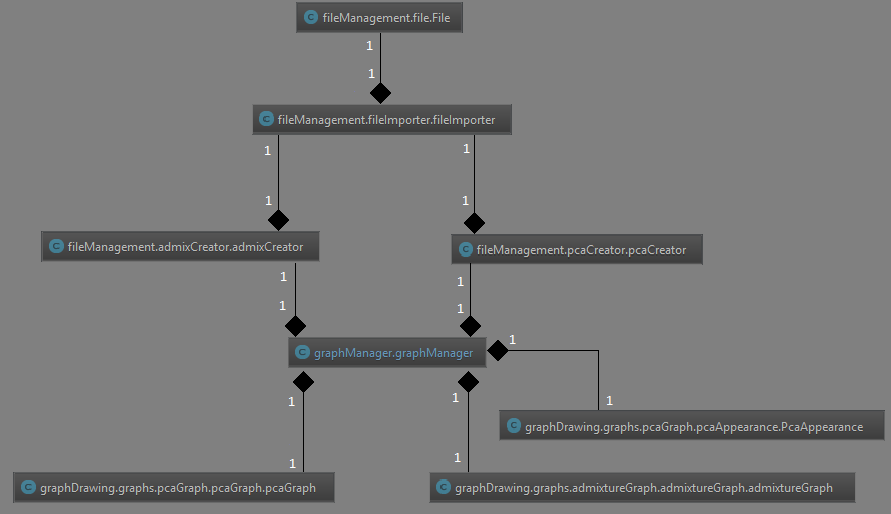
\includegraphics[scale = 0.65]{regenesis_class_precursor.png}
\caption{ReGenesis Class Diagram}
\label{rgf class diagram}
\end{figure}

\subsubsection{File}
This class is responsible for storing data and metadata of a file including the file type and file name.

\subsubsection{pcaGraph}

This class is responsible for storing individuals, their coordinates and their groups for the PCA plot. It also stores appearance settings for the graph. 

\subsubsection{admixGraph}

This class is responsible for storing individuals, their ancestral proportions and their population groups for the structure plot.

\subsubsection{graphManager}
This class is the central controller for ReGenesis. It controls all other classes directly or indirectly via the other controller classes. This class also acts as the view for ReGenesis. This violates the MVC architecture, however this choice was made as all of the view functionality is implemented using external libraries. As such, it was deemed that separating this class into two would unnecessarily complicate the design and increase the time cost of the project.

\subsubsection{pcaCreator}
This class provides an interface for the importing of the files required for a PCA plot. This class also controls the fileImporter.

\subsubsection{admixCreator}
This class provides an interface for the importing of the files required for a structure plot. This class also controls the fileImporter.

\subsubsection{fileImporter}
This class is responsible for interfacing with the file system as well as generating a File object for the parent Creator object.

\subsubsection{pcaAppearance}

This class provides an interface for the user to edit the appearance of a pcaGraph object. Currently the user can change the colour, shape and size of each group of individuals. The user can also set a title and choose whether to show grid-lines and axis-labels.
\end{document}

%%% Local Variables: 
%%% mode: latex
%%% TeX-master: t

%%% End: 
